\section{Web Scraping with R}\label{web-scraping-with-r}

\subsection{An introduction for
beginners}\label{an-introduction-for-beginners}

Feng Li\\
feng.li@cufe.edu.cn

\subsection{Outline}\label{outline}

\begin{itemize}
\tightlist
\item
  Why web scraping?
\item
  What researchers do with web data?
\item
  How to scrape web data?
\end{itemize}

\subsection{Why web scraping?}\label{why-web-scraping}

\subsection{Why do we need Web
Scraping?}\label{why-do-we-need-web-scraping}

\begin{itemize}
\item
  Data on the web is growing exponentially.
\item
  If the only way you access the Internet is through a browser, you're
  missing out on a huge range of possibilities.
\item
  Rather than viewing one page at a time, you can access thousands or
  even millions of pages at once.
\item
  If you can view it in your browser
  \textbackslash{}(\textbackslash{}Rightarrow\textbackslash{}) you can
  access it via a script
  \textbackslash{}(\textbackslash{}Rightarrow\textbackslash{}) you can
  store it in a database
  \textbackslash{}(\textbackslash{}Rightarrow\textbackslash{}) you can
  do virtually anything with that data.
\end{itemize}

\subsection{\texorpdfstring{A practical application:
\href{https://www.wefeelfine.org}{``We Feel
Fine''}}{A practical application: We Feel Fine}}\label{a-practical-application-we-feel-fine}

\begin{itemize}
\tightlist
\item
  Project by Jonathan Harris and Sep Kamvar.
\item
  Scraped a variety of English-language blog sites for phrases starting
  with ``I feel'' or ``I am feeling''.
\item
  Describe how the world was feeling day by day and minute by minute.
\end{itemize}

\subsection{\texorpdfstring{``We Feel
Fine''}{We Feel Fine}}\label{we-feel-fine}

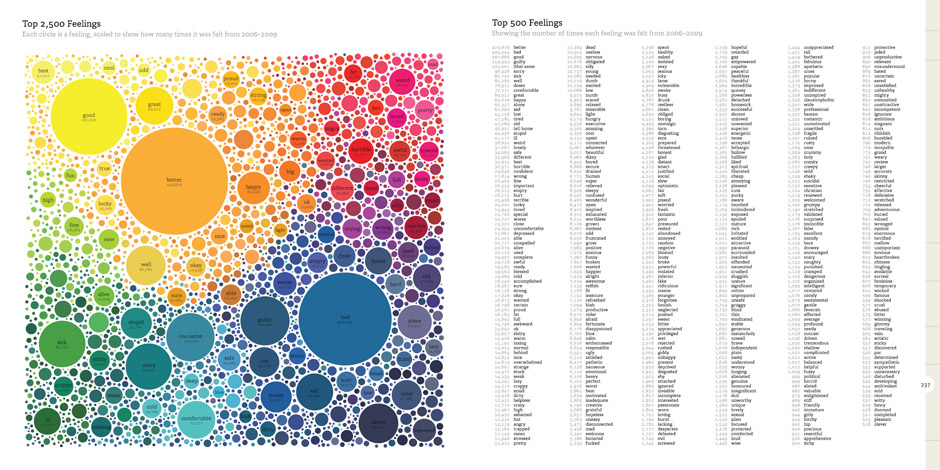
\includegraphics[width=10.41667in,height=5.20833in]{treemap-big.jpg}

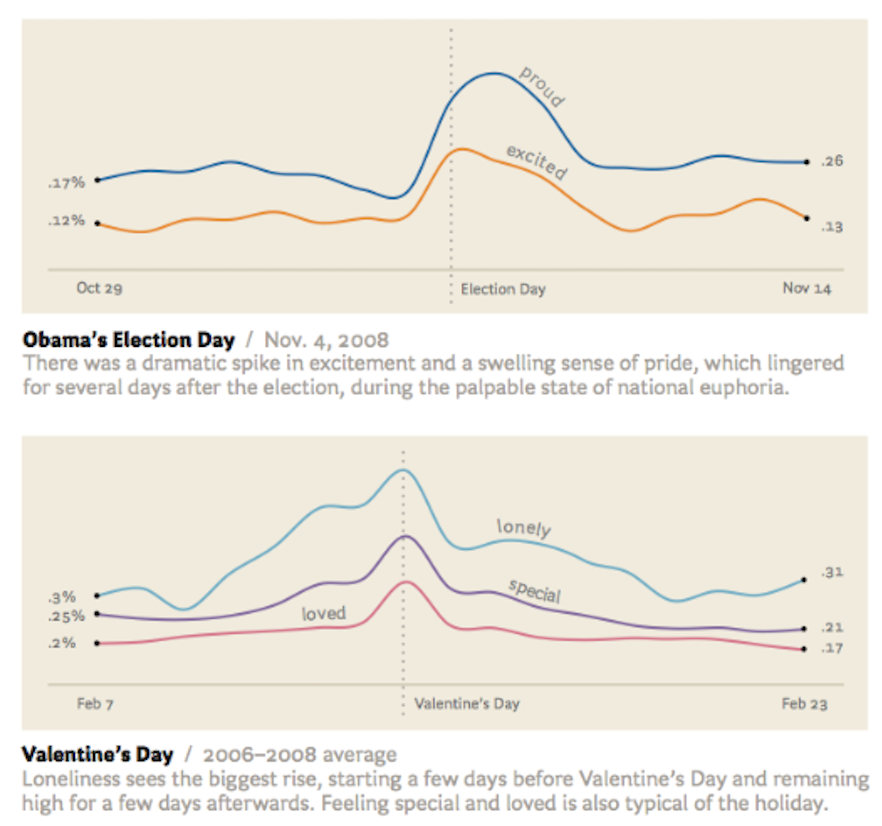
\includegraphics[width=5.20833in,height=4.68750in]{emotionTS1.png}

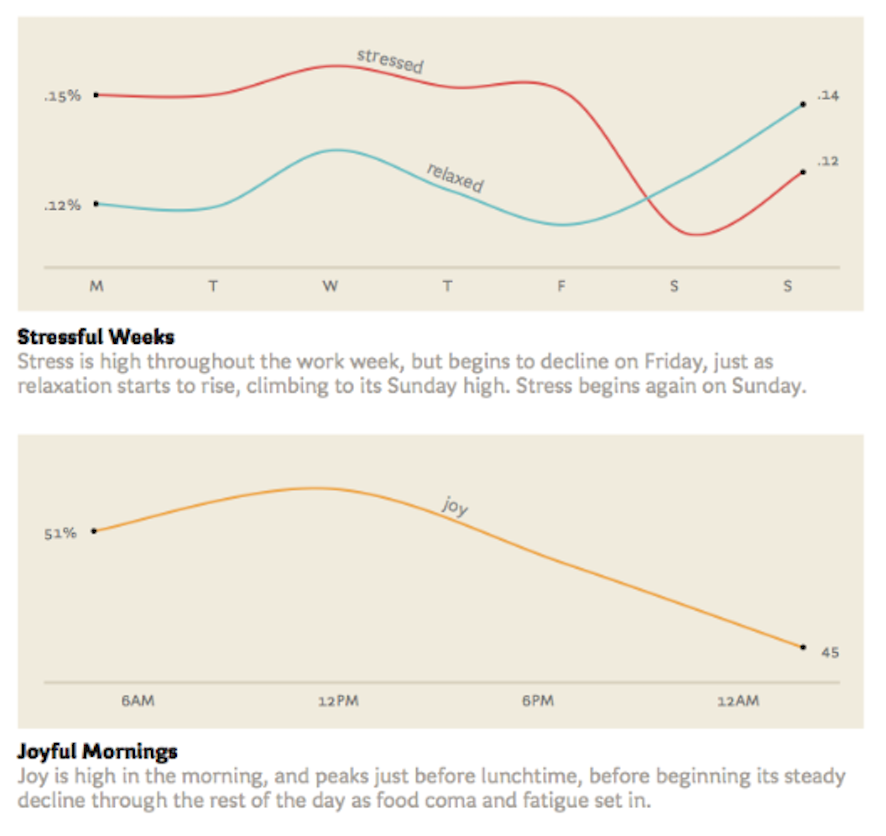
\includegraphics[width=5.20833in,height=4.68750in]{emotionTS2.png}

\subsection{What researchers do with web
data?}\label{what-researchers-do-with-web-data}

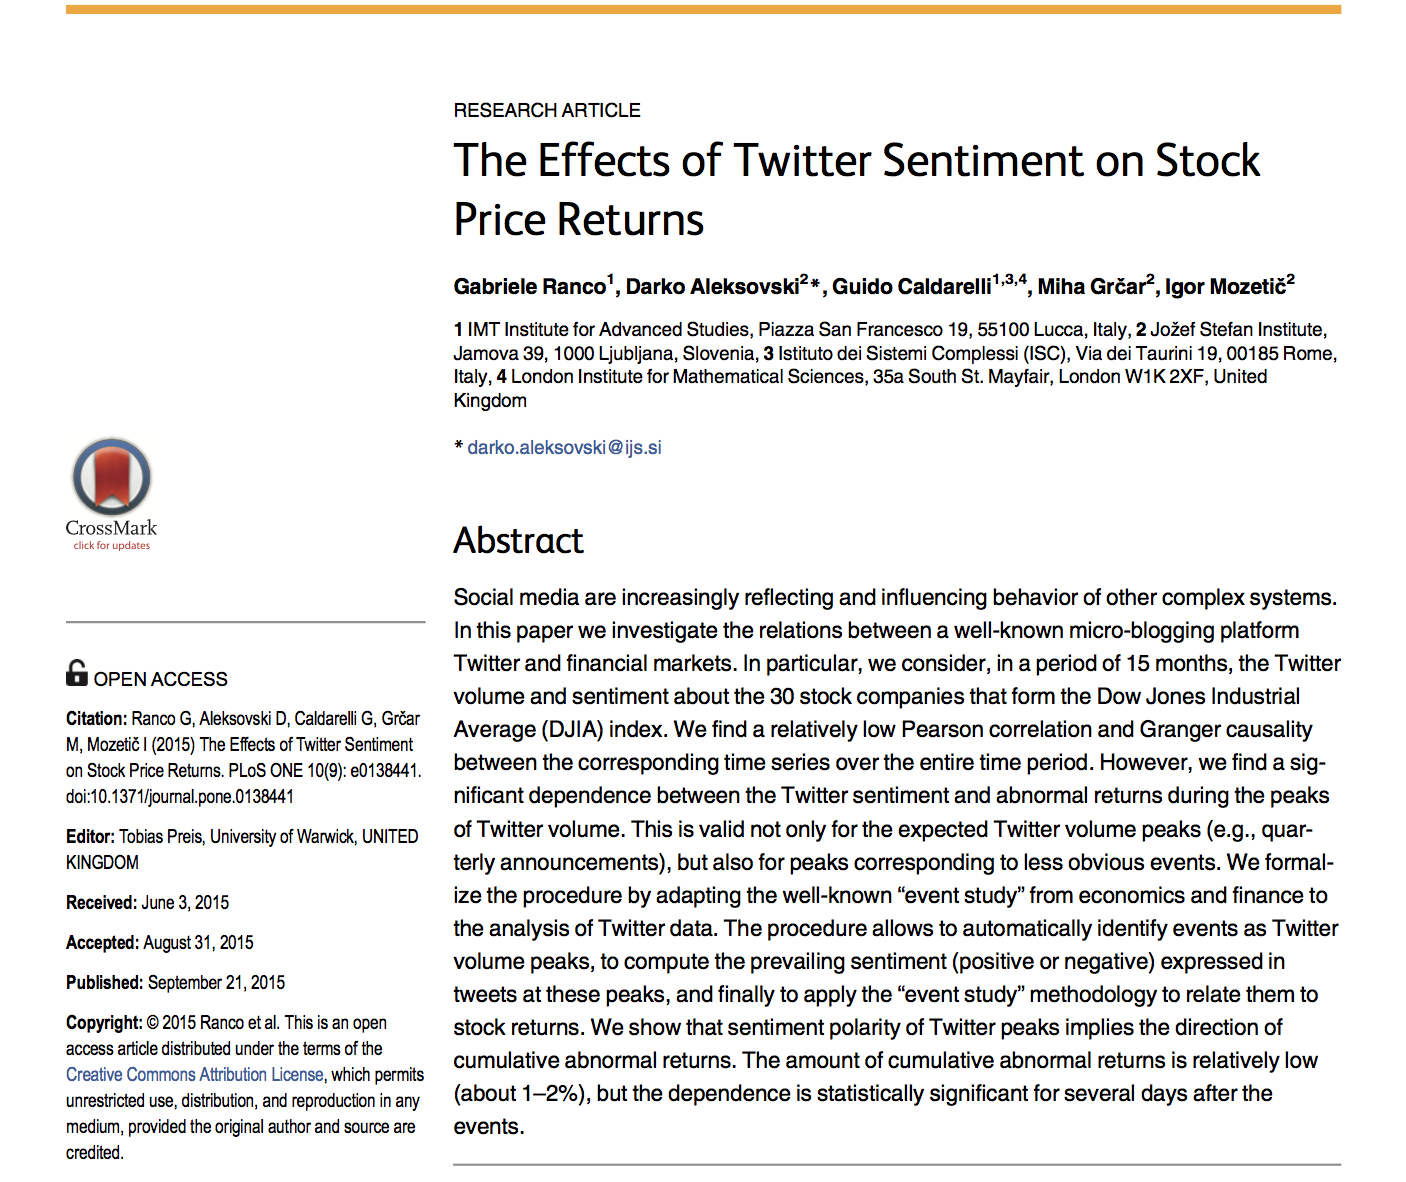
\includegraphics[width=7.81250in,height=6.45833in]{twitter1.png}


\includegraphics[width=7.81250in,height=6.25000in]{twitter.png}

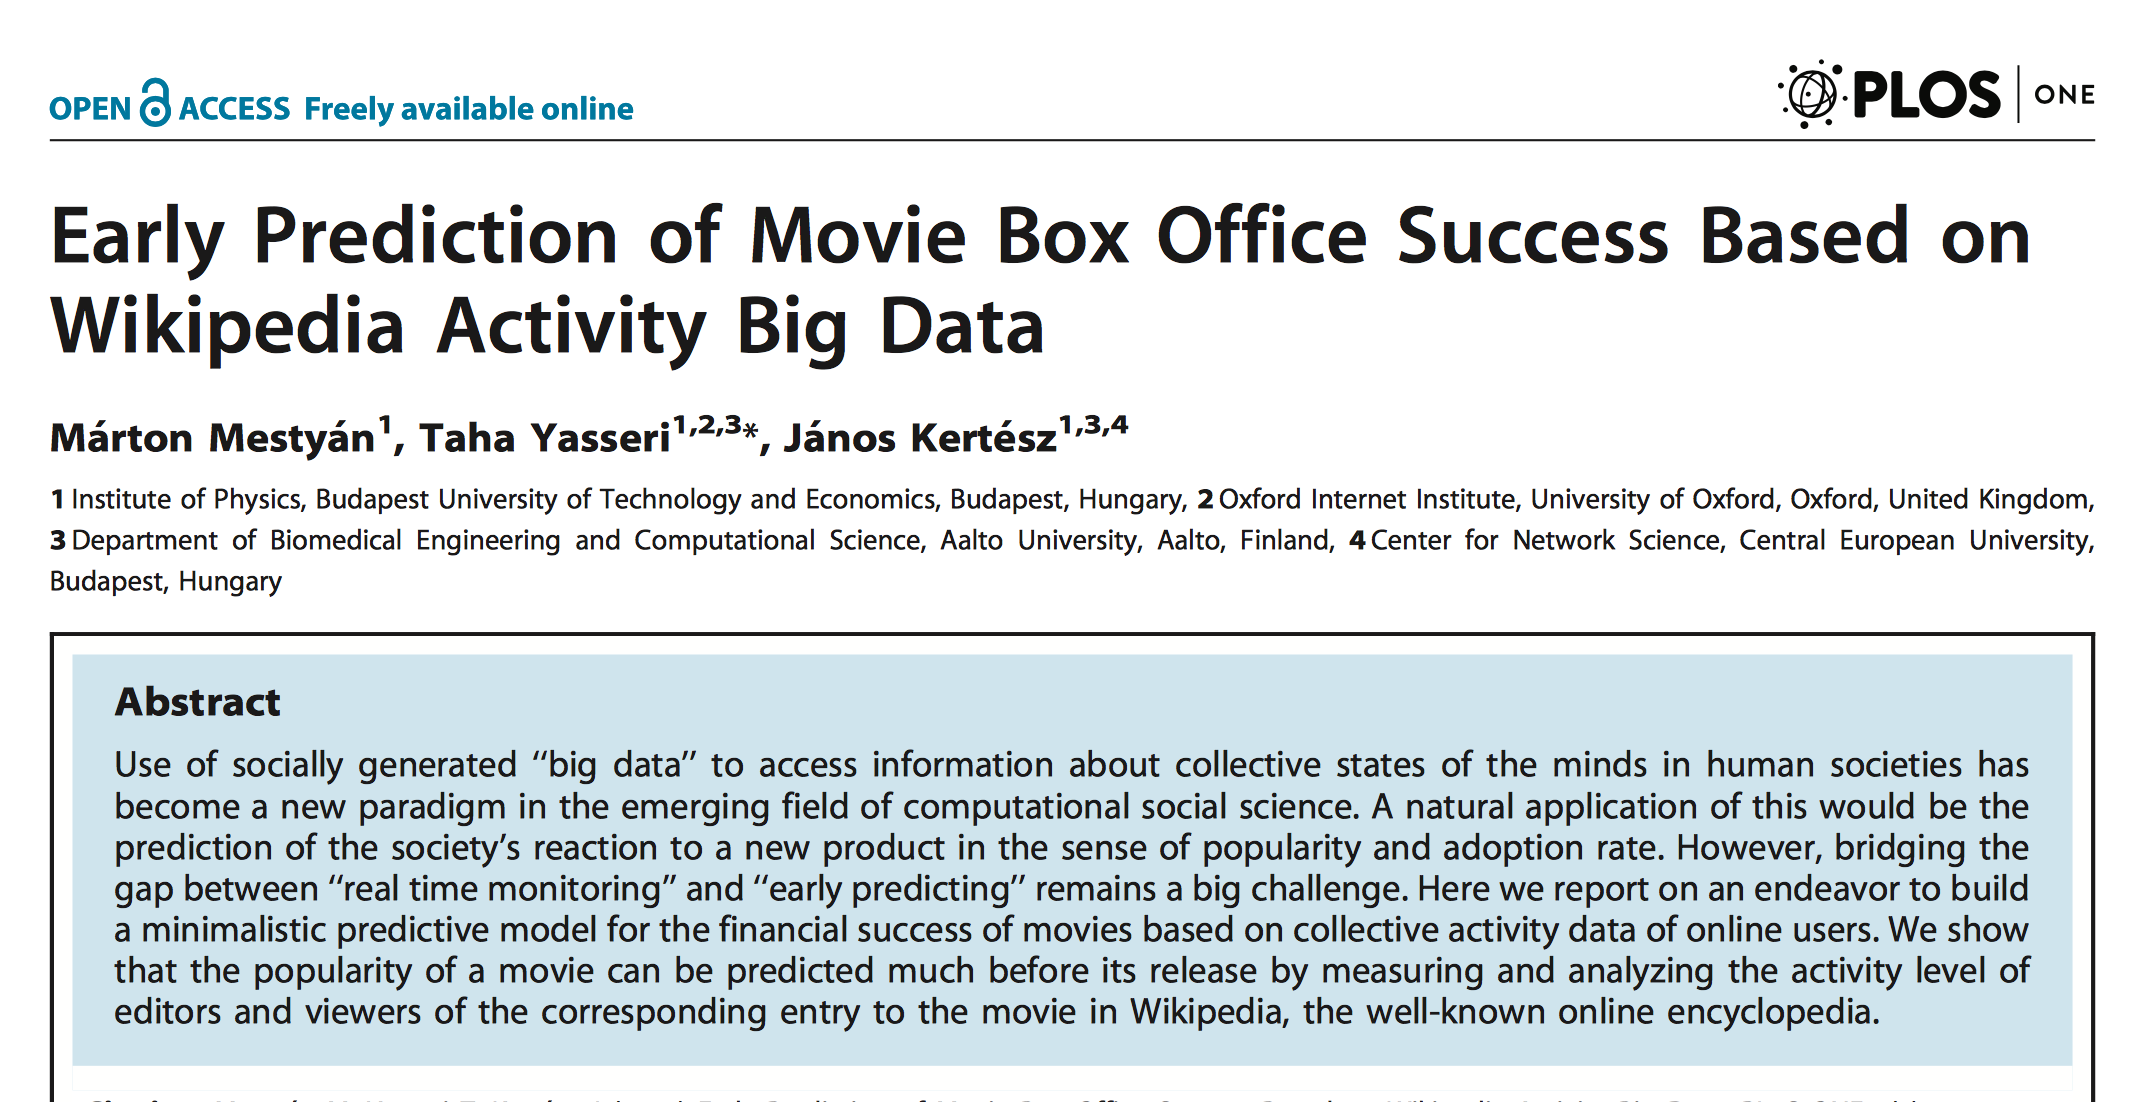
\includegraphics[width=9.89583in,height=5.72917in]{movie.png}


\includegraphics[width=9.89583in,height=4.16667in]{google.png}

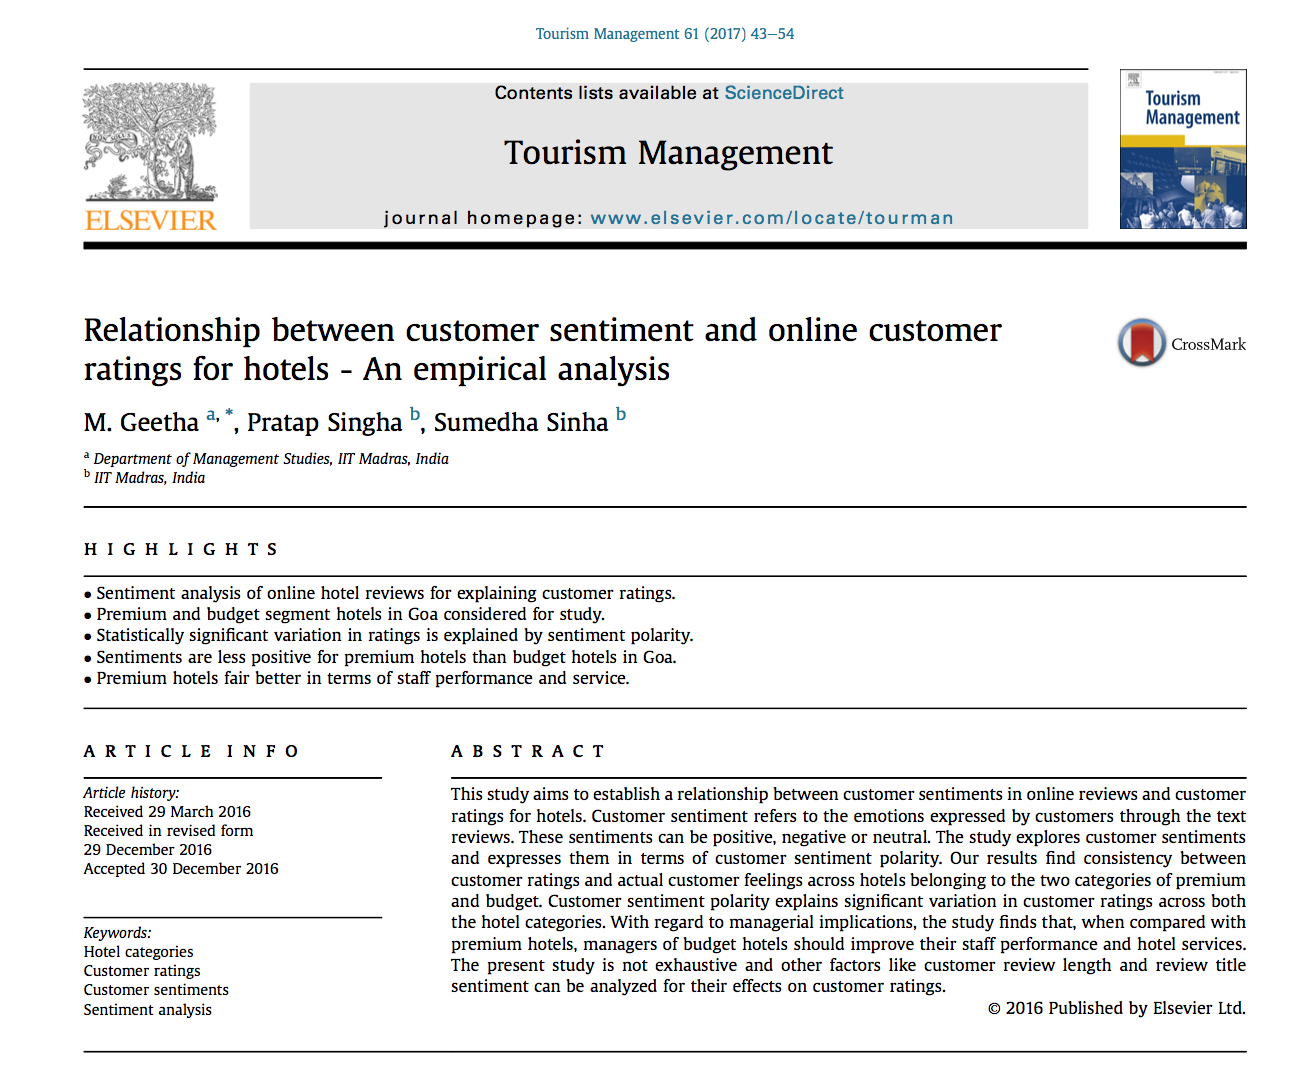
\includegraphics[width=7.60417in,height=6.45833in]{hotel.png}


\includegraphics[width=7.29167in,height=6.77083in]{sales1.png}

\subsection{But web data is messy!}\label{but-web-data-is-messy}

Most of the web data is not readily available. It is present in an
unstructured format (HTML format).

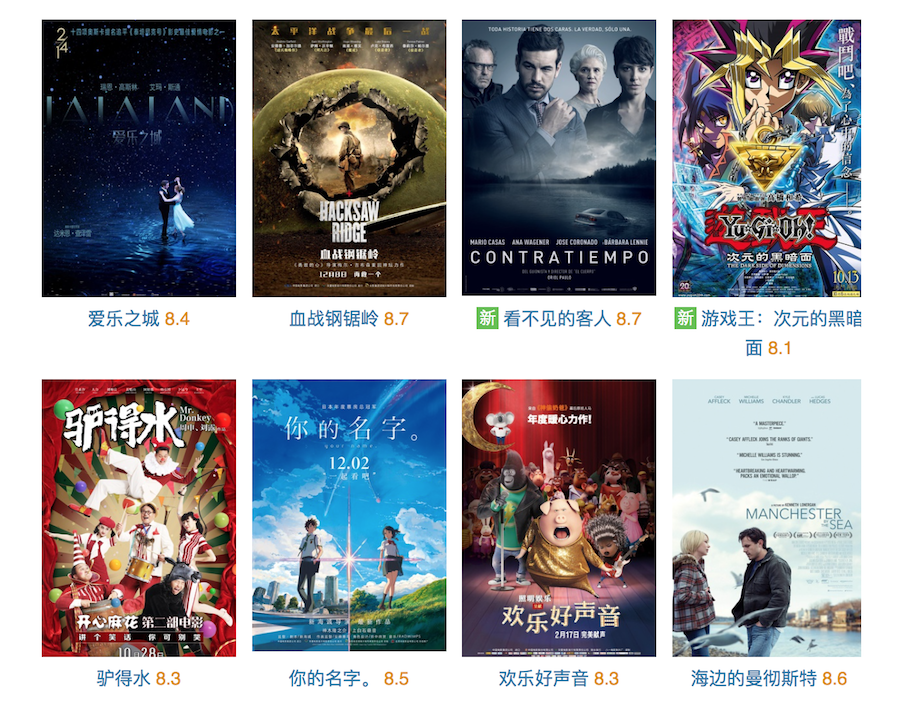
\includegraphics[width=5.20833in,height=4.06250in]{douban.png}

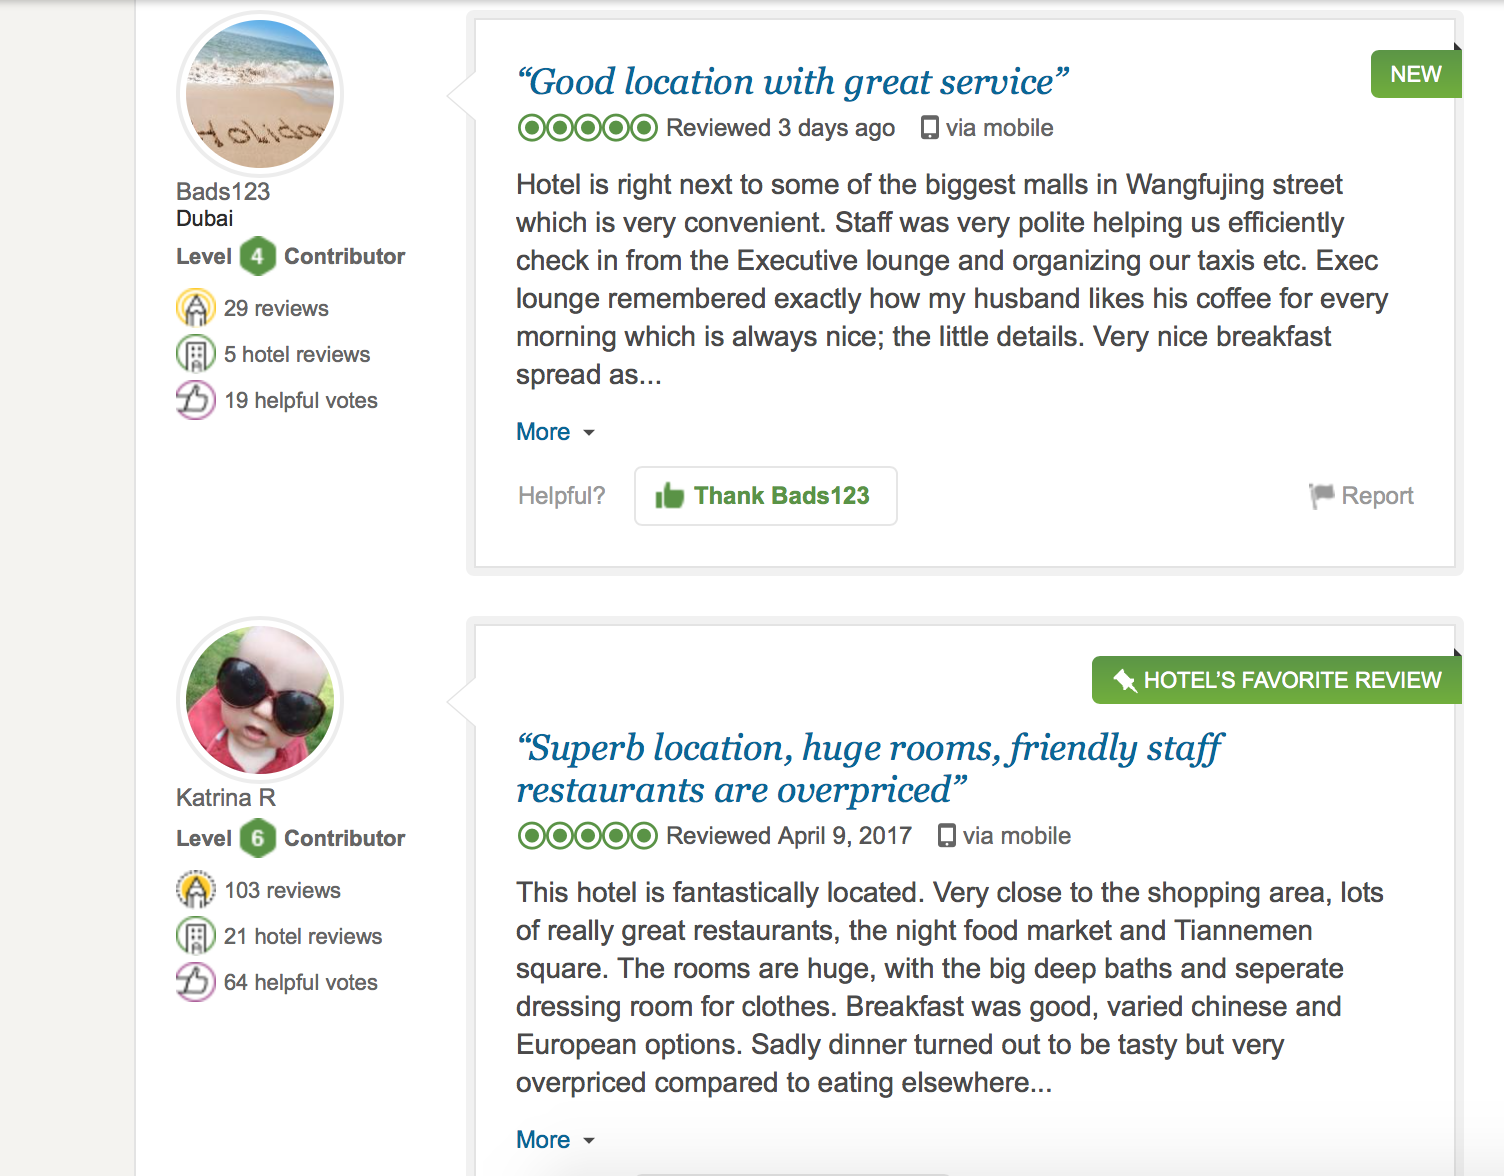
\includegraphics[width=5.20833in,height=4.06250in]{HotelReview.png}

\subsection{Data we really want}\label{data-we-really-want}

But we want a tidy format of data!

\begin{itemize}
\tightlist
\item
  rows == observations
\item
  columns == attributes
\end{itemize}

\begin{longtable}[]{@{}llll@{}}
\toprule
Movie & Score & Length (mins) & Language\tabularnewline
\midrule
\endhead
爱乐之城 & 8.4 & 128 & English\tabularnewline
看不见的客人 & 8.7 & 106 & Spanish\tabularnewline
\ldots{} & \ldots{} & \ldots{} & \ldots{}\tabularnewline
\bottomrule
\end{longtable}

\subsubsection{\texorpdfstring{\textbf{Web scraping expertise
required!}}{Web scraping expertise required!}}\label{web-scraping-expertise-required}

\subsection{How to scrape web data?}\label{how-to-scrape-web-data}

\subsection{Get familiar with the structure of a html
(tags)}\label{get-familiar-with-the-structure-of-a-html-tags}

\begin{itemize}
\item
  When we do web scraping, we deal with html tags to find the path of
  the information we want to extract.
\item
  A simple html source code: tree structure of html tags. HTML tags
  normally come in pairs.
\end{itemize}

\begin{verbatim}
<!DOCTYPE html>
<html>
  <title> My title
  </title>
  <body>
    <h1> My first heading </h1>
      <p> My first paragraph </p>
  </body>
</html>
\end{verbatim}

\subsection{Work with other useful
tags}\label{work-with-other-useful-tags}

\begin{itemize}
\item
  HTML links are defined with the \texttt{\textless{}a\textgreater{}}
  tag
  \texttt{\ \textless{}a\ href="http://www.test.com"\textgreater{}This\ is\ a\ link\ for\ test.com\textless{}/a\textgreater{}}
\item
  HTML tables are defined with \texttt{\textless{}table\textgreater{}},
  row as \texttt{\textless{}tr\textgreater{}} and rows are divided into
  data as \texttt{\textless{}td\textgreater{}}
\item
  HTML list starts with \texttt{\textless{}ul\textgreater{}} (unordered)
  and \texttt{\textless{}ol\textgreater{}} (ordered). Each item of list
  starts with \texttt{\textless{}li\textgreater{}}
\item
  Try \url{http://www.tryiteditor.com} to learn more about html.
\end{itemize}

\subsection{XPath}\label{xpath}

\begin{itemize}
\item
  When we do web scraping, we use XPath to locate the piece of data we
  want.
\item
  Path used to select nodes and info in html.
\item
  One of the most crucial step to do web scraping.
\end{itemize}

\begin{verbatim}
<!DOCTYPE html>
<html>
  <title> My title
  </title>
  <body>
    <h1> My first heading </h1>
      <p> My first paragraph </p>
  </body>
</html>
\end{verbatim}

\begin{itemize}
\tightlist
\item
  \texttt{/html/title}: selects the
  \texttt{\textless{}title\textgreater{}} element of an HTML document
\item
  \texttt{//p}: selects all the \texttt{\textless{}p\textgreater{}}
  elements
\end{itemize}

\subsection{XPath}\label{xpath-1}

\begin{verbatim}
<html> 
  <head>
    <title>Example website</title> 
  </head>
  <body>
    <div id='images', class='img'>
      <a href='image1.html'>Name: Image 1<img src='image1_thumb.jpg'/></a> 
      <a href='image2.html'>Name: Image 2<img src='image2_thumb.jpg'/></a> 
    </div> 
  </body>
</html>
\end{verbatim}

\begin{itemize}
\item
  \texttt{//div{[}@id="images"{]}}: selects all the
  \texttt{\textless{}div\textgreater{}} elements which contain an
  attribute \texttt{id="images"}.
\item
  \texttt{//div{[}@id="images"{]}/a/}: selects all the
  \texttt{\textless{}a\textgreater{}} elements inside the aforementioned
  element.
\end{itemize}

\subsection{XPath}\label{xpath-2}

\begin{verbatim}
<td class="zwmc" style="width: 250px;">
  <div style="width: 224px;*width: 218px; _width:200px; float: left">
    <a style="font-weight: bold">金融分析师</a>
  </div>
</td>
\end{verbatim}

\begin{itemize}
\tightlist
\item
  \texttt{//td{[}@class="zwmc"{]}/div/a}
\item
  \texttt{//td{[}@class="zwmc"{]}//a}
\end{itemize}

\subsection{Where to go?}\label{where-to-go}

scrape job information from \url{http://sou.zhaopin.com} of jobs related
to `阿里巴巴'.

\begin{itemize}
\item
  Inspect a web page (easily found in Chrome).
\item
  Find the xpath for the elements you want to extract

  \begin{itemize}
  \tightlist
  \item
    E.g., xpath for job titles: \texttt{//td{[}@class="zwmc"{]}/div/a}.
  \item
    You can also find xpath from viewing the whole page source
  \end{itemize}
\end{itemize}

\subsection{Scrapping a webpage using rvest package in
R}\label{scrapping-a-webpage-using-rvest-package-in-r}

\begin{itemize}
\tightlist
\item
  Parse the entire website: \texttt{read\_html()}.
\item
  Find and extract the pieces of the website you need using XPath:
  \texttt{html\_nodes()}. It pull out the entire node.
\item
  The following are done after using html\_nodes() to extract content we
  need.

  \begin{itemize}
  \tightlist
  \item
    \texttt{html\_table()}: extract all data inside a html table.
  \item
    \texttt{html\_text()}: extract all text within the node.
  \item
    \texttt{html\_attr()}: extract contents of a single attribute.
  \item
    \texttt{html\_attrs()}: extract all attributes.
  \end{itemize}
\item
  Cleanup
\end{itemize}

\subsection{Go back to previous
examples}\label{go-back-to-previous-examples}

\begin{verbatim}
web <- read_html('<!DOCTYPE html>
<html>
  <title> My title
  </title>
  <body>
    <h1> My first heading </h1>
      <p> My first paragraph </p>
  </body>
</html>')
title_node <- html_nodes(web, xpath = '//title')
# html_text(title_node)
str_trim(html_text(title_node))
\end{verbatim}

\begin{verbatim}
## [1] "My title"
\end{verbatim}

\subsection{Now we want to scrape data from a html
table}\label{now-we-want-to-scrape-data-from-a-html-table}

\begin{verbatim}
url <- "https://en.wikipedia.org/wiki/Provinces_of_China"
web <- read_html(url)
provinces_nodes <-
  html_nodes(web, xpath = '//*[@class="wikitable sortable"]')
provinces <- html_table(provinces_nodes)
\end{verbatim}

\begin{longtable}[]{@{}lllllllll@{}}
\toprule
GB{[}2{]} & ISO{[}3{]} & Province & Chinese Hanyu Pinyin & Capital &
Population1 & Density2 & Area3 & Abbreviation4\tabularnewline
BJ & CN-11 & Beijing Municipality & 北京市Běijīng Shì & Beijing &
19,612,368 & 1,167.40 & 16,800 & 京Jīng\tabularnewline
TJ & CN-12 & Tianjin Municipality & 天津市Tiānjīn Shì & Tianjin &
12,938,224 & 1,144.46 & 11,305 & 津Jīn\tabularnewline
HE & CN-13 & Hebei Province & 河北省Héběi Shěng & Shijiazhuang &
71,854,202 & 382.81 & 187,700 & 冀Jì\tabularnewline
SX & CN-14 & Shanxi Province & 山西省Shānxī Shěng & Taiyuan & 35,712,111
& 228.48 & 156,300 & 晋Jìn\tabularnewline
NM & CN-15 & Inner Mongolia Autonomous Region & 內蒙古自治区Nèi Měnggǔ
Zìzhìqū & Hohhot & 24,706,321 & 20.88 & 1,183,000 & 內蒙古(蒙)Nèi Měnggǔ
(Měng)\tabularnewline
\bottomrule
\end{longtable}

\subsection{Now scrape some employment
data}\label{now-scrape-some-employment-data}

\begin{verbatim}
library(rvest)
url <- 'http://sou.zhaopin.com/jobs/searchresult.ashx?jl=北京&kw=阿里巴巴'
web <- read_html(url)
job_title_nodes <- html_nodes(web, xpath = '//td[@class="zwmc"]/div/a')
job_title <- html_text(job_title_nodes)
job_title[1:2]
\end{verbatim}

\begin{verbatim}
## [1] "阿里妈妈-java研发专家-北京"   "大文娱-APP推广-PP助手&豌豆荚"
\end{verbatim}

\begin{verbatim}
link <- html_attr(job_title_nodes, 'href')
link[1:2]
\end{verbatim}

\begin{verbatim}
## [1] "http://jobs.zhaopin.com/000127917285693.htm"     
## [2] "http://jobs.zhaopin.com/00012791790284592000.htm"
\end{verbatim}

\subsection{Pipeable!}\label{pipeable}

\begin{verbatim}
job_title_nodes <- html_nodes(web, xpath = '//td[@class="zwmc"]/div/a')
job_title <- html_text(job_title_nodes)
\end{verbatim}

\textbackslash{}(\textbackslash{}Downarrow\textbackslash{})

\begin{verbatim}
job_title <- web %>%
  html_nodes(xpath = '//td[@class="zwmc"]/div/a') %>%
  html_text()
\end{verbatim}

\subsection{Let's extract more data}\label{lets-extract-more-data}

\begin{verbatim}
url <- 'http://sou.zhaopin.com/jobs/searchresult.ashx?jl=北京&kw=阿里巴巴'
web <- read_html(url, encoding = "utf-8")
job_title <- web %>%
  html_nodes(xpath = '//td[@class="zwmc"]/div/a') %>% html_text()
link <- web %>%
  html_nodes(xpath = '//td[@class="zwmc"]/div/a') %>% html_attr('href')
company <- web %>%
  html_nodes(xpath = '//td[@class="gsmc"]') %>% html_text()
salary <- web %>%
  html_nodes(xpath = '//td[@class="zwyx"]') %>% html_text()
location <- web %>%
  html_nodes(xpath = '//td[@class="gzdd"]') %>% html_text()
alibaba_jobs <- data.frame(job_title, company, salary, location, link)
\end{verbatim}

\begin{longtable}[]{@{}lllll@{}}
\toprule
job\_title & company & salary & location & link\tabularnewline
\midrule
\endhead
阿里妈妈-java研发专家-北京 & 阿里巴巴集团 & 面议 & 北京 &
http://jobs.zhaopin.com/000127917285693.htm\tabularnewline
大文娱-APP推广-PP助手\&豌豆荚 & 阿里巴巴集团 & 面议 & 北京 &
http://jobs.zhaopin.com/00012791790284592000.htm\tabularnewline
大文娱-SEM优化师-UC & 阿里巴巴集团 & 面议 & 北京 &
http://jobs.zhaopin.com/00012791790284591000.htm\tabularnewline
大文娱-广告平台优化师-UC & 阿里巴巴集团 & 面议 & 北京 &
http://jobs.zhaopin.com/00012791790284967000.htm\tabularnewline
大文娱-app推广-UC & 阿里巴巴集团 & 面议 & 北京 &
http://jobs.zhaopin.com/00012791790284968000.htm\tabularnewline
大文娱-运营优化师-终端 & 阿里巴巴集团 & 面议 & 北京 &
http://jobs.zhaopin.com/00012791790285570000.htm\tabularnewline
\bottomrule
\end{longtable}

\subsection{How to turn pages?}\label{how-to-turn-pages}

Think about how to turn pages.

\subsection{Extract more job details via its
link}\label{extract-more-job-details-via-its-link}

\begin{verbatim}
get_job_detail <- function(link){
  link = as.character(link)
  web = read_html(link)
  experience = web %>%
    html_nodes(xpath ='//ul[@class="terminal-ul clearfix"]/li[5]/strong') %>% html_text()
  degree = web %>%
    html_nodes(xpath ='//ul[@class="terminal-ul clearfix"]/li[6]/strong') %>% html_text()
  number = web %>%
    html_nodes(xpath ='//ul[@class="terminal-ul clearfix"]/li[7]/strong') %>% html_text()
  description = web %>%
    html_nodes(xpath ='//div[@class="terminalpage-main clearfix"]/div/div[1]')%>% html_text()
  description = str_trim(sub('查看职位地图', '', description))
  link_details = data.frame(experience, degree, number, description)
  return(link_details)
}
\end{verbatim}

\subsection{Extract more job details via its
link}\label{extract-more-job-details-via-its-link-1}

\begin{verbatim}
job_details <- data.frame()
for (i in 1:nrow(alibaba_jobs)){
  job_details = rbind(job_details, get_job_detail(alibaba_jobs$link[i]))
}
alibaba_job_details <- cbind(alibaba_jobs, job_details)
kable(head(subset(alibaba_job_details, select = -c(link,description))), format = "html")
\end{verbatim}

\begin{longtable}[]{@{}lllllll@{}}
\toprule
job\_title & company & salary & location & experience & degree &
number\tabularnewline
\midrule
\endhead
阿里妈妈-java研发专家-北京 & 阿里巴巴集团 & 面议 & 北京 & 3-5年 & 本科 &
若干\tabularnewline
大文娱-APP推广-PP助手\&豌豆荚 & 阿里巴巴集团 & 面议 & 北京 & 3-5年 &
本科 & 若干\tabularnewline
大文娱-SEM优化师-UC & 阿里巴巴集团 & 面议 & 北京 & 3-5年 & 本科 &
若干\tabularnewline
大文娱-广告平台优化师-UC & 阿里巴巴集团 & 面议 & 北京 & 3-5年 & 本科 &
若干\tabularnewline
大文娱-app推广-UC & 阿里巴巴集团 & 面议 & 北京 & 3-5年 & 本科 &
若干\tabularnewline
大文娱-运营优化师-终端 & 阿里巴巴集团 & 面议 & 北京 & 5-10年 & 本科 &
若干\tabularnewline
\bottomrule
\end{longtable}

\subsection{Practice if you like}\label{practice-if-you-like}

\begin{itemize}
\item
  Extract at least 5 attributes of the movies listed on Douban top 250
  (\url{https://movie.douban.com/top250})
\item
  Extract the top 5 pages of hotel information including the newest
  reviews from TripAdvisor
  (\url{https://www.tripadvisor.com/Hotels-g294212-Beijing-Hotels.html})
\item
  Extract the top 5 pages of book information from Amazon
  (\href{https://www.amazon.cn/s/ref=nb_sb_noss?__mk_zh_CN=\%E4\%BA\%9A\%E9\%A9\%AC\%E9\%80\%8A\%E7\%BD\%91\%E7\%AB\%99\&field-keywords=\%E5\%A4\%A7\%E6\%95\%B0\%E6\%8D\%AE}{https://www.amazon.cn/s/ref=nb\_sb\_noss?\_\_mk\_zh\_CN=亚马逊网站\&field-keywords=大数据})
\end{itemize}

\subsection{Some notes}\label{some-notes}

\begin{itemize}
\item
  When you scrape a website too frequently, the server may reject your
  request. One possible solution is to stop for several seconds
  irregularly.
\item
  Not every website is scrappable! Some websites go with really high
  technoloy to protect their data from being extracted. For example,
  they use javascript, or really complex captcha codes.
\item
  Python has more functionality for web scraping. It is more flexible to
  deal with the problems mentioned above. If you are interested in that,
  please refer to
  \href{https://yanfei.site/docs/dpsa/references/PyWebScrapingBook.pdf}{this
  book}. Basics of web scraping with Python are similar.
\end{itemize}

\subsection{References}\label{references}

\begin{itemize}
\tightlist
\item
  \href{https://cran.r-project.org/web/packages/rvest/rvest.pdf}{\texttt{rvest}}
\item
  \href{https://en.wikibooks.org/wiki/R_Programming/Text_Processing}{Wikibooks
  on text processing}
\end{itemize}

\subsection{Further readings}\label{further-readings}

\begin{itemize}
\tightlist
\item
  Other packages like \texttt{XML}, \texttt{RCurl} and \texttt{scrapR}
  are also used for web scraping
\item
  \href{https://yanfei.site/docs/dpsa/references/PyWebScrapingBook.pdf}{Web
  Scraping with Python}
\end{itemize}

\subsection{Questions?}\label{questions}


\includegraphics[width=7.29167in,height=5.20833in]{thanks.jpg}

\hypertarget{io2012-ptoc}{}
\begin{itemize}
\tightlist
\item
  \protect\hyperlink{}{1}
\item
  \protect\hyperlink{}{2}
\item
  \protect\hyperlink{}{3}
\item
  \protect\hyperlink{}{4}
\item
  \protect\hyperlink{}{5}
\item
  \protect\hyperlink{}{6}
\item
  \protect\hyperlink{}{7}
\item
  \protect\hyperlink{}{8}
\item
  \protect\hyperlink{}{9}
\item
  \protect\hyperlink{}{10}
\item
  \protect\hyperlink{}{11}
\item
  \protect\hyperlink{}{12}
\item
  \protect\hyperlink{}{13}
\item
  \protect\hyperlink{}{14}
\item
  \protect\hyperlink{}{15}
\item
  \protect\hyperlink{}{16}
\item
  \protect\hyperlink{}{17}
\item
  \protect\hyperlink{}{18}
\item
  \protect\hyperlink{}{19}
\item
  \protect\hyperlink{}{20}
\item
  \protect\hyperlink{}{21}
\item
  \protect\hyperlink{}{22}
\item
  \protect\hyperlink{}{23}
\item
  \protect\hyperlink{}{24}
\item
  \protect\hyperlink{}{25}
\item
  \protect\hyperlink{}{26}
\item
  \protect\hyperlink{}{27}
\item
  \protect\hyperlink{}{28}
\item
  \protect\hyperlink{}{29}
\item
  \protect\hyperlink{}{30}
\item
  \protect\hyperlink{}{31}
\item
  \protect\hyperlink{}{32}
\item
  \protect\hyperlink{}{33}
\item
  \protect\hyperlink{}{34}
\item
  \protect\hyperlink{}{35}
\item
  \protect\hyperlink{}{36}
\item
  \protect\hyperlink{}{37}
\end{itemize}
